\documentclass[conference]{IEEEtran}

\IEEEoverridecommandlockouts
% The preceding line is only needed to identify funding in the first footnote. If that is unneeded, please comment it out.
\usepackage{cite}
\usepackage{amsmath,amssymb,amsfonts}
\usepackage{algorithmic}
\usepackage{graphicx}
\usepackage{textcomp}
\usepackage{xcolor}
\usepackage{listings}
\graphicspath{{./images/}}
\def\BibTeX{{\rm B\kern-.05em{\sc i\kern-.025em b}\kern-.08em
    T\kern-.1667em\lower.7ex\hbox{E}\kern-.125emX}}
\begin{document}

\title{A Decentralized Pub/Sub System for Trusted Machine Economy}

\author{\IEEEauthorblockN{1\textsuperscript{st} Ching-Hua (Vivian) Lin}
\IEEEauthorblockA{\textit{dept. of CSIE} \\
\textit{National Cheng Kung University}\\
Tainan City, Taiwan (R.O.C.) \\
jkrvivian@gmail.com}
\and
\IEEEauthorblockN{2\textsuperscript{nd} Ching-Chun (Jim) Huang}
\IEEEauthorblockA{\textit{dept. of CSIE} \\
\textit{National Cheng Kung University}\\
Tainan City, Taiwan (R.O.C.) \\
jserv@ccns.ncku.edu.tw}
\and
\IEEEauthorblockN{3\textsuperscript{rd} Chia-Heng Tu}
\IEEEauthorblockA{\textit{dept. of CSIE} \\
\textit{National Cheng Kung University}\\
Tainan City, Taiwan (R.O.C.) \\
chiaheng@gmail.com}
}

\maketitle

\begin{abstract}

\end{abstract}

\begin{IEEEkeywords}
Data Marketeplace, decentralization, Distributed Ledger Technology
\end{IEEEkeywords}

\section{Introduction}
%TODO: cite examples
In Internet of Things (IoT), the development of machine-to-machine (M2M) technology\cite{M2M}, cyber physical system (CPS)\cite{CPS} and Industry 4.0 grow rapidly. As the physical and digital data are deeply intertwined, the interactions among digital twins act as data exchanges\cite{digitaltwin} which brings a potential value to IoT applications, such as health care\cite{healthCare}, factories and vehicles\cite{AutonomousDriving}, and brings up new business models where data is considered as tradeable digital assets. With the diverse data streams generated by different entities and carried accross organizations among expanding amount of interconnected devices, it is a challenge for data holders to share and track their data assets. Therefore, data marketplace is viewed as a solution to build a secure, reliable and scalable data sharing platform where data providers and data consumers meet.  

Among the challenges of data marketplace\cite{BigDataMarket}, our proposed decentralized data marketplace in\cite{MyDataMarketplace} focuses on the following issues:

\begin{itemize}
	\item \textbf{Scalability}. 
1) The performance of data marketplace should scale with the massive amount of participants. 2) Keys managed by participants should be as small as possible. 
	\item \textbf{Integrity}. 1) Prevent unauthorized modifications. 2) Ensure the accuracy and validity of contents.	
	\item \textbf{Confidentiality}. 
1) Only the authorized participants can access data streams. 2) Participants that have access can always retrieve data even if they're dropped from the network.	
	\item \textbf{Privacy}. 1) Avoid revealing sensitive information of all participants, such as IP address and data consumers' habits which may leaked within the subscription history.
	\item \textbf{Economics Incentive}. The economics incentives can encourage the data providers to participate the system and pay more attention on the quilatiy control. 
\end{itemize}




% may be removed
The publish-subscribe messaging model is widely used in IoT applications for exchanging data between devices due to its scalability and resource-effieciency. In the publish-subscribe system, a broker is the bridge to meet publishers and subscribers. Broker is a centralized group that arrange the communication between the publishers and subscribers. However, the centralized architecture brings potential vulnerabilities and security issues:

\begin{enumerate}
	\item Central point of failure. 
	The broker is usually held by a single organization. If the centralized server is crashed or attacked, the services will not be available. 	
	\item Data integrity.
	As broker controls the interaction between publishers and subscribers, an unreliable or compromised broker can easily tamper data streams. 
	\item Anonymity and privacy.
	Broker matches publishers and subscribers in order to relay data streams to corresponding entities. The unreliable broker can expose the subscribers' interests and personal information of both entities.  
\end{enumerate}
  


 
\section{Related Work}
The publish/subscribe service model consists of publishers, subscribers and brokers, which has been proven\cite{pubSubAnalysis, pubSubAnalysis2} to be an efficient and flexible solution for a large number of diverse entities like IoT applications. A lot of work in publish/subscribe system focused on the scalability and the different security issues such as, encrypted data communication, privacy preserving data subscription and access control of digital asset. A few work targets on the storage which is a vital considerations for IoT and mobile computing and the incentive for data economics.

M. B. Abdullahi and G. Wang\cite{centralPubSub} presented a secure publish/subscribe data storage service in Wireless sensor networks (WSNs) which ensures several security issues. Each user has an identity for authentication, whereas subscribers' interests are encoded before matching to protect users' interests. Additionally, the proposed encryption scheme can prevent adversary to access published data if the sensor node is compromised. However, the access control and encryption keys of data is enforced by the network controllers (NCs) and Cirtificate Authorities (CAs), which may be a potential security risk of the system. Also the storage is not well illustrated in the work. G. S. Ramachandran et al.\cite{trinity} pointed out the security risk of centralized brokers, and applied DLTs to build a distributed pub/sub system which promotes the transparency of interactions of participants and the status of data. With the help of Smart Contract, usesrs can perform data validation easily, and brokers can keep track of data status. But data is plaintext on blockchain, which the privacy problem of sensitive data need to be considered carefully. The economics incentives that can encourage the publishers to participate the system and pay more attention on the quilatiy control are not included. 

In \cite{userCentricData}, the publisher runs a node in blockchain that preserves all the history data of the ledger, therefore, they can publish and manage data without any third-parties. The subscribers request publisher directly and ask them to save a cache space for interested data. The main contribution of the system is to ensure data owners have full controls of produced data, but the data owners need to have well devices and environment to perform such functionalities and preserve data. Also, the rights for accessing digital assets is more compatible in the IoT scenarios instead of copying raw data. Secure Pub-Sub model\cite{SPS}, a brokerless of publish/subscribe model, is proposed to eliminate the security risk of middlewares in the model and to provide a reputation-based fairness payment strategy on blockcahin. The privacy and data security are considered thoroughly with the encryption scheme, while the reputation of publishers, payment and data sharing are deployed on smart contracts that allows all operations are transparent. The reputation system and the punishment rules against malicous acts of subscribers and publishers. Yet, without brokers, providers and subscribers may need to reveal more sensitive information like IP address in order to match the both sides. Another broker-less model in \cite{PrivacyPreservPubSub} protects the subscribers' privacy by encrypting users' interests with the light-weight PKEwET\cite{PKEwET}, which allows publishers to match the subscribers' interests in cipher text. 

Decentralized storage systems allow users to store files in a distributed network that is maintained by individual nodes around the world instead of a central service provider. Nevertheless, DLTs are often used as the backbone of these systems as data storage and also an incentive layer to encourage people get involved in the network. Filecoin \cite{FileCoin} in Inter-Planetary File system(IPFS)\cite{IPFS} is an incentive layer to incent nodes to provide storage. IPFS is a content-based addressing storage model in a peer-to-peer network, which users can obtain the data with the unique hash value through the network. However, no cryptographic system is applied for user-uploaded files. Sia\cite{Sia} splits the uploaded file into multiple data segments encrypted with the owner's private key, then cipher text is sent to the Sia nodes that rent the storage in Siacoin through smart contracts. Files are duplicated in multiple nodes to prevent data loss.
 
\section{System Architecture}
The proposed data subscription framework\cite{MyDataMarketplace} is a decentralized architecture with data providers, data subscribers and brokers that interact between data providers and subscribers, including data publishment, product metadata generation and trading process.

\subsection{Participants}
There are three major roles in the decentralized data marketplace (Fig.~\ref{fig:system_design}).

\begin{itemize}
\item \textbf{Data Provider: }
Data providers generate and preserve streaming data, and are willing to provide streaming data to subscribers. Providers can use the subscription fee paid by subscribers to improve the quality of their service.
\item \textbf{Subscribers: }
Subscribers aspire to obtain streaming data to promote the value of their service. However, it is a significant challenge for most subscribers to collect the desired data by themselves, so they look to purchasing the streaming data from data providers.
\item \textbf{Broker: }
Brokers represent data providers and subscribers to perform blockchain computing tasks and are expected to have higher resource. The brokers are requested to handle the product launching and subscription process, and brokerage fees is charged in each process.
\end{itemize}

\begin{figure}[!t]
    \centering
    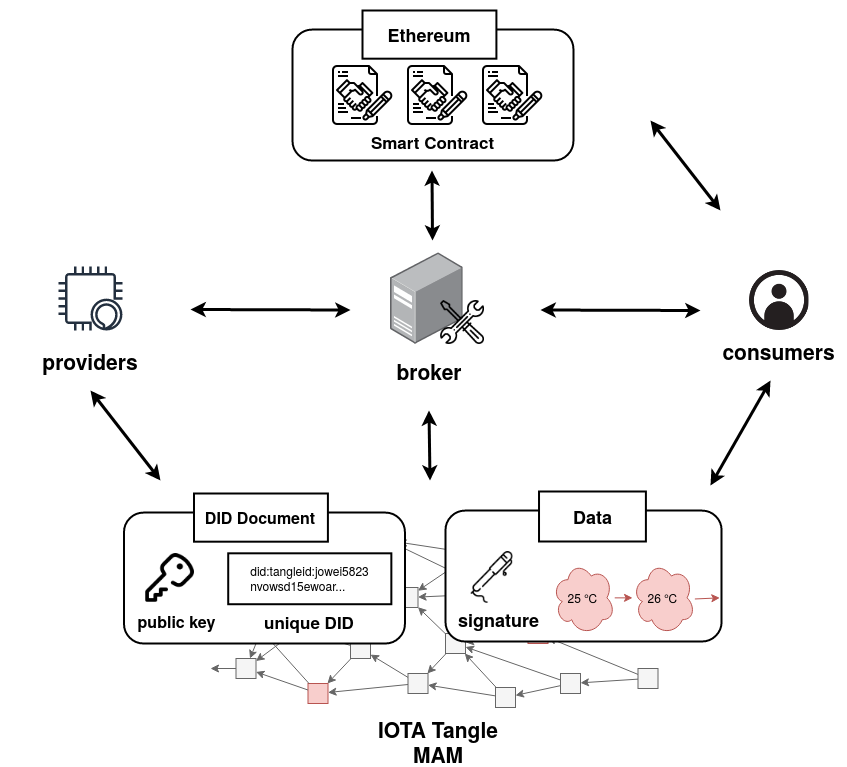
\includegraphics[width=3.in]{system_design}
    \caption{The system design of a decentralized architecture which consists of data providers, subscribers and brokers.}
    \label{fig:system_design}
\end{figure}

\subsection{Components}
There are several building blocks in the proposed design to meet the expectations: 1) emit and access encrypted data stream; 2) retrieve transaction data for audit; 3) digital identity for all participants; and 4) enforcement of transparency and traceability.


\subsubsection{Masked Authenticated Messaging}
IOTA is a feeless cryptocurrency designed for IoT while MAM is the second layer data communication protocol built on top of the IOTA network, the Tangle. MAM resolves the challenge of publishing authenticated streaming data as zero-value transactions to distributed ledgers, and provides the ability to publish and fetch encrypted messages over the Tangle along with data integrity and access control.
With MAM, the rights of accessing data is traded instead of a copy of data itself, which gives a flexibilty for subscribers to obtain data anywhere anywhen that subscribers do not need additional storage to store the data it buy.
 
In the IOTA protocol, seed is the identifier of its owner. An IOTA seed represents the ownership of all things associated with the user in the IOTA ecosystem, such as IOTA tokens or messages on the Tangle. With the seed, the owner can produce addresses and signatures in order to issue transactions or publish messages to MAM channels and endpoints.

Either channel or endpoint is like a singly-linked list. The MAM channel ID and endpoint ID are the addresses of transaction and are the root of a channel and endpoint. Each address of a message can be derived from the previous one. A user can create multiple channels and multiple endpoints under the same channel. The messages can be encrypted with the session key and broadcasted in chronological order to the Tangle by attaching it to an endpoint. This allows only entities that know the session key to be able to decode these messages after retrieving them from the Tangle, and the singly-linked list structure implements the concept of forward secrecy, where anyone has no access to the data back from his/her entry point. Fig.~\ref{fig:mam_struct} shows the architecture of MAM.

\begin{figure}[!t]
    \centering
    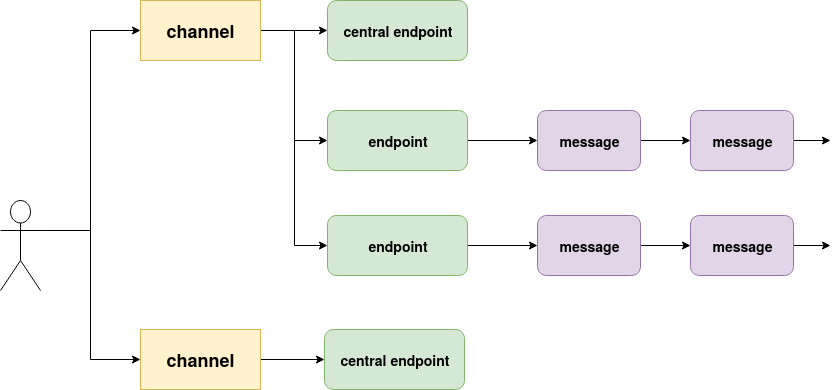
\includegraphics[width=2.5in]{mam_struct}
    \caption{The concept of MAM.}
    \label{fig:mam_struct}
\end{figure}

The authentication in MAM includes source and data authentication. Source authentication ensures that the message originates from the claimed owner, and data authentication ensures the integrity of the data from that sender. These are achieved through the Merkle signature scheme\cite{MSS} (MSS) which is a digital signature scheme based on Merkle Hash Trees and One-way hash functions. However, the size of Merkle Hash Trees should be fixed at start, which is the size of a channel and the endpoint is decided before creation. Thus, data providers need to firstly decide how to distribute data product into MAM channels or endpoints.

%use case illustration
Data providers are the primary role to interact with the MAM. With a seed, a provider can start creating a channel and endpoint. As mentioned above, the length of a channel and an endpoint is fixed, thus providers need to decide the selling unit of data products according to their data type or pricing strategy. Also data providers can a make product preview which is public and not encrypted on MAM. In Fig.~\ref{fig:mam_struct}, a "central endpoint" means its endpoint's ID is the same as channel's ID. By attaching part of the product to central endpoint can give subscribers a quick preview with channel's ID only, and users can easily verify the content with digital signatures in messages. Then if the trade is established, providers can then give subscribers the encrypted endpoint and session key to subscribers.
 
The decentralized and fault-tolerant characteristic of distributed ledgers reduce the risks of centralized storage services, and the underlying IOTA network is scalable which withstands real-time data while increasing users all over the world. Moreover, the features of MAM make it an even better data storage which allows preserving streaming data while ensuring data integrity, proving data ownership to any participants and managing session keys of data. And through the access control and the protocol of MAM, participants are allowed to subscribe to the future data. This ensures that only service requester and selected provider are in possession of a key to decrypt and read the content of the MAM channel and therefore retrieve transaction data for audit.

While the operations of MAM are time-consuming, brokers are responsible not only for being the bridge between providers and subscribers, but also for all MAM related operations, such as channel creation and encrypted data publishing in our system. See Fig.~ \ref{fig:launching_product}.

\begin{figure}[!t]
    \centering
    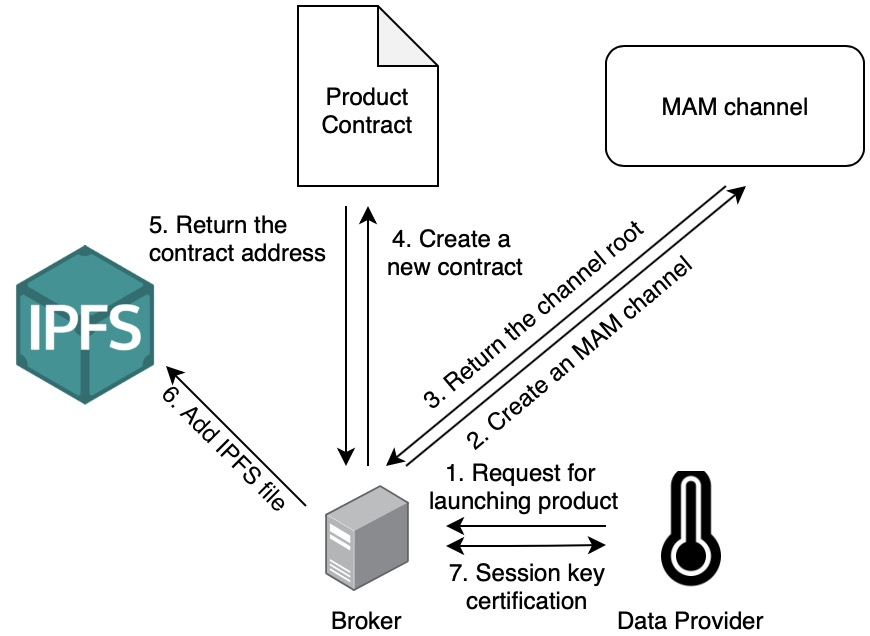
\includegraphics[width=2.5in]{launching_product}
    \caption{The process of launching a product.}
    \label{fig:launching_product}
\end{figure}

\subsubsection{TangleID}
The TangleID\cite{TangleID} is a self-sovereign identity system based on IOTA that does not require any third-party authority to verify an identity and its digital footprint. With TangleID, the digital footprint is converted into digital assets under the principle of Decentralized Identifiers (DIDs)\cite{DID} defined by W3C. Posting DID documents on MAM channel makes TangleID a GDPR-compliant system\cite{GDPR}. Every participant in the data marketplace registers on TangleID, hence one can easily verify data providers' identity to ensure the data persistency from data sources.

A public/private key pair and an IOTA seed are generated in TangleID. The public MAM channel is created with the seed and its MAM channel ID becomes part of the unique user ID, which at the same time serves as DID with the purpose of publishing the public key of the entity. Private key along with the IOTA seed is stored in the local database of the entity. The public/private key pair can be used in secure message sharing within users and digital signature.

The digital identities are also used to establish trust between the communication partners. This is done on two levels to prove that the communication partner owns the DID and the partner can, optionally, proof that it is a trusted participant. This authentication process happens during the first messages of interaction. In order for one partner to listen to another, it authenticates the messages. The DID ownership authentication is done by proving a digitally signed copy of the DID document.

The authentication of trust between the two parties is based on a Verifiable Credential, given out by a trusted issuer for the receiving party. If the receiving party does not trust the issuer, the credential is deemed worthless. If the party is recognized, the credential is verified and the messages will be labelled as trusted. In order to acquire this credential, the party needs to contact the issuer and ask for the credential. The issuer will need to know the DID of the party. If they decide to give out the credential, the issuer will sign the credential and send it encrypted over the blockchain to the requesting party's communication address. This is listed as a Service Endpoint (DID standard) in the DID Document of the requesting party.

\subsubsection{Ethereum Smart Contract}
The smart contract is a protocol for formulating agreement on a blockchain that provides verification and execution of the contract. The code in the smart contract can interact with other contracts, make decisions, store data and transfer cryptocurrency. All conditions and states established in the contract are transparent and enforceable. The appearance of smart contracts makes trading more flexible, and achieves more complex trading patterns in reality.

The Product Contract is used during the trading process, where Product Contract records all the details of data products, such as MAM channel's and endpoint's ID, blinded session key and data providers' DID Document address. Furthermore, data providers and subscribers exchange session keys through a Product Contract without involving brokers. Though this design may cost more in transaction fees than doing so off-chain, it is considered a better strategy to assure the profit of both providers and subscribers. The further details of key exchangement will be illustrated in Section~\ref{section:trading}.

\subsubsection{Blind Signature}
There is an inherent risk in revealing session keys to brokers since contents may be copied by brokers, which would result in data providers' losses. Therefore, a blind signature is used to prevent session key copying for such circumstances. A blind signature\cite{blindSig} is a form of digital signature where the message is first "blinded" by a random "blinding factor", then passed to a signer to sign. Fig.~\ref{fig:blind_signature} illustrates the steps of blind signature. The resulting message, along with the blinding factor, can be later verified with the signer's public key. In our system design, brokers would perform blind signatures during the process of adding new products for data providers, in order to send the secret key of the MAM channel to the smart contract without knowing it.

\begin{figure}[!t]
	\centering
	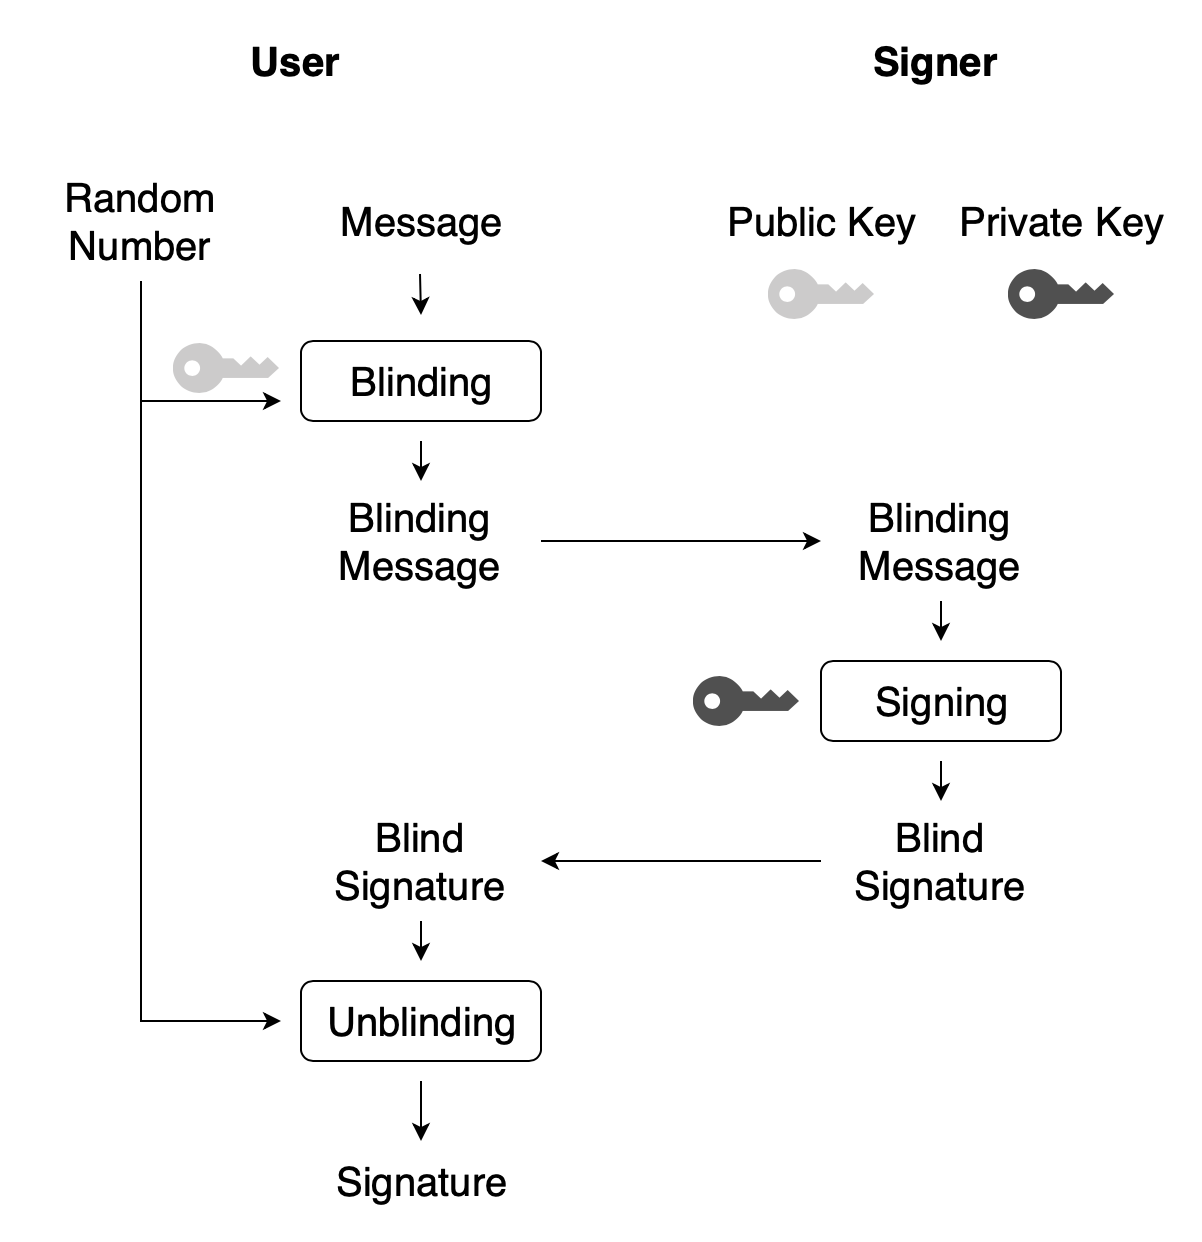
\includegraphics[width=2. in]{blind_signature}
	\caption{The scheme of blind signature.}
	\label{fig:blind_signature}
\end{figure}

RSA blind signature\cite{cryptoNote} is used in our research. The user chooses a random number $r$ and uses the signer's public key $e$ to generate a blinding factor $r^e$. To prevent the message $m$ from being known by the signer, the user sends blinding message $c$ to the signer instead of $m$.

\begin{equation}
C = r^e m
\end{equation}

The signer signs the blinding message with private key $d$.

\begin{equation}
S = C^d
\end{equation}

$S$ is the signer's signature of $C$. In RSA system, $ed$ is equal to 1. To remove the blinding factor, the user computes the following calculation.

\begin{equation}
\frac{S}{r}= \frac{C^d}{r} = \frac{(r^e m)^d}{r} = \frac{r^{ed} m^d}{r} = m^d
\end{equation}
 
The user gets $m^d$ which is the signer's signature of the message $m$. At the same time, the signer does not know $m$ and the session key is protected. 

\section{Trading Model}
In the following, we describe the data trading process in detail. To participate a data marketplace, data providers and subscribers have to first register. Then,  the data provider can launch its product on the marketplace. Once a product is launched, it is searchable on IPFS where brokers upload the information of the product and can be subsequently traded. The whole trading and refunding process is defined in smart contracts which are easily traceable and irreversible.

\subsection{Set up}
At the beginning, all participant need to register on TangleID in order to get a DID document and public/private key pairs. The DID document is shared within the following operations to perform authentication, key exchangement and secure communication. 

\subsection{Trading}
\label{section:trading}

The entire trading process is as shown in Fig.~\ref{fig:trading_product}. Once a subscriber wants to subscribe certain streaming data that is generated, he/she has to pay subscription fee to the Product Contract and will be automatically added to the subscriber list by the smart contract.

\begin{figure}[!t]
    \centering
    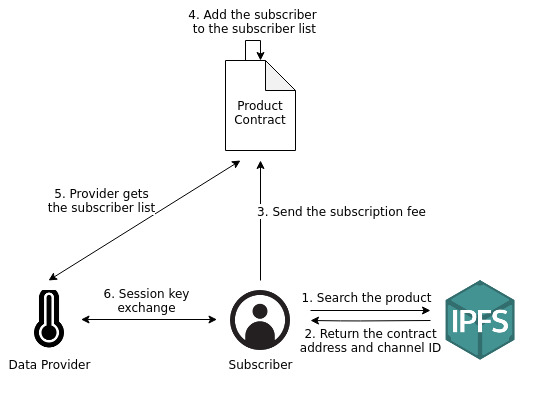
\includegraphics[width=2.5in]{trading_product}
    \caption{The process for the product trading.}
    \label{fig:trading_product}
\end{figure}

In the proposed architecture, the "access" to specific data stream is traded instead of giving out the raw data copies. Subscribers can retrieve data on MAM at any time without equipping extra storage to preserve data, and one can also query for arbitrary section of data rather downloading them all. Thus, the most important part of trading process is to give the session key $k$, the encryption key of data stream, to the subscribers. In order to exchange data, Azaria et al\cite{Medrec} seek an off-chain solution which is based on an end-to-end communication to ensure the efficiency and low costs. However, it is hard to avoid that the data source is unavailable or the sender sends incorrect data intentionally. Instead of the off-chain solution, we use smart contract to transfer the session key\cite{3tierDataMarket} that not only ensures the consistency of the session key, the availability of the source and the traceability of the record, but also prevents malicious participants to cheat others. With the help of brokers and smart contracts, both providers and subscribers do not need to be online at the same time to proceed the trading process.

\lstdefinestyle{solidity}{
	captionpos=b,
	tabsize=4,
	basicstyle=\scriptsize
}
\lstset{style=solidity}

\begin{lstlisting}[caption={Update encryption key}, label={lst:key_exchange}, frame=single]
function addEncryptKey(
  address _subscriber,
  string memory _encryptKey
) public {
  require(
      msg.sender == provider,
      "Only provider can add blindedKey."
  );
  require(
      subscriber2Purchase[_subscriber].isKeyAdded == false,
      "One encryptKey has been added."
  );
  subscriber2Purchase[_subscriber].encryptKey = _encryptKey;
  subscriber2Purchase[_subscriber].isKeyAdded = true;
  emit newEncryptKey(_subscriber, _encryptKey);
}
\end{lstlisting}

The trading process is shown in Fig.~\ref{fig:key_exchange}. The data provider can obtain public keys of each subscriber from the DID document. For each subscriber, the data provider encrypts the session key and broker's signature with the subscriber's public key and sends the ciphertext $Encrypt(k + Sign(k))$ to the product contract by calling $addEncryptKey()$ (Listing \ref{lst:key_exchange}). Subscribers listen to the $newEncryptKey$ event which is triggered when the ciphertext is updated, and decrypt the ciphertext to obtain the session key $k$ and signature $Sign(k)$.

\begin{figure}[!t]
    \centering
    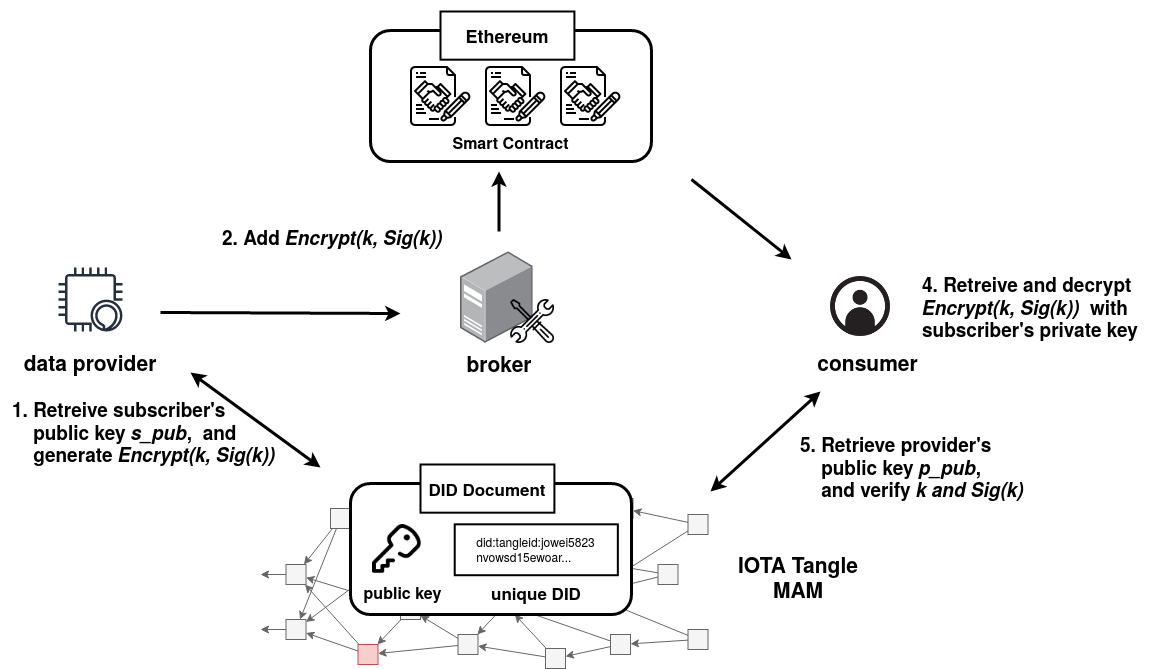
\includegraphics[width=3.5in]{key_exchange}
    \caption{Session key exchange process between the data provider and subscriber.}
    \label{fig:key_exchange}
\end{figure}

Subscribers can obtain the broker's public key on the DID document as well, so they can verify that the validation of signature and the session key is the only one certified by the broker. Afterward, with the MAM channel ID and session key $k$, subscribers can obtain the data.

\subsection{Refunding}

It is probable that the streaming data sources are delayed or even interrupted after the subscribers pay the subscription fee. To protect subscriber rights, the subscription fee are not transferred to the data provider until data is generated and published to the MAM channel. If the expected data is not available, subscribers can request refunds. We assume that a very small percentage of subscribers in the product contract are irrational and/or malicious. When a subscriber consents to refund, he can vote at any time. After the ratio of consent votes of refunding is higher than the $threshold$, the subscription fee is proportionally transferred to the data provider, broker and every subscriber. Fig.~\ref{fig:refund} shows the refund process.

\begin{figure}[!t]
	\centering
	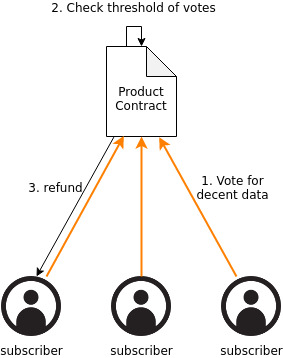
\includegraphics[width=1.5in]{refund}
	\caption{The process of refund.}
	\label{fig:refund}
\end{figure}

The subscription fee can be prorated as below:

\begin{equation}
    F_{DataProvider}(i) = N price \frac{i-1}{M} (1-F_{b}) -F_{t}
\end{equation}

\begin{equation}
    F_{Broker}(i) = N price \frac{i-1}{M} F_{b} -F_{t}
\end{equation}

\begin{equation}
    F_{Subscriber}(i) = price \frac{M-i+1}{M} -F_{t}
\end{equation}

where $i$ is the number of data when refunding condition is met, $price$  is the subscription price, $M$ is the number of expected data samples, $F_{b}$ (\%) is the brokerage fee which is expressed as a percentage, $F_{t}$ is the transaction fee of the smart contract, $N$ is the number of subscribers in this contract.

To refund or withdraw subscription fees from the smart contract, the data provider, broker, and subscriber send a transaction to execute the smart contract and are responsible for the transaction fee. We assume that only a half of the expected records are published to the MAM channel. When $F_{b}$ is 5\%, the data provider and broker can withdraw half of the total subscription fee from the smart contract and 5\% of the subscription fee belongs to the broker while the remaining belongs to the data provider. For subscribers, they can receive half of the subscription fee refunded which should be deducted from the transaction fee.

Considering the situation that one of the subscribers requests a refund in the future, when the subscriber is disappointed with the data quality, he/she may request a refund.

\section{Evaluations}
It is worth making a claim that all participants in data marketplace do not need to hold an IOTA full node which maintains the transaction history and exchanges information of the Tangle. Each role is only required to run client libraries and communicate with IOTA full nodes to interact with the Tangle. Therefore, in the following evaluations, all devices run with client library only.

\subsection{MAM Performance Evaluation}
MAM is a secure and validatable data storage of the proposed architecture. And publishing data to MAM is the primary key to resolve all the difficulties discussed in previous sections. The interactions between data providers and MAM can be frequent. Data providers can either upload data in a short time interval or maintain multiple MAM channels or endpoints at the same time, hence the operation of MAM is one of the potential bottleneck in data marketplace.

In this section, time measurement is evaluated in two MAM operations: channel/endpoint creation and data attachment to endpoints. To perform the evaluation assessment, a personal computer (PC, 3.2GHz 64-bit 6-core i7-8700 with 16GB DDR4 RAM) and a Raspberry Pi 3 Model B (1.2 GHz 64-bit quad-core ARM Cortex-A53 with 1GB LPDDR2 RAM) have been used to run MAM. 

\subsubsection{Channel / Endpoint Creation}
The length of a channel or endpoint is $2^{height}-1$ where \textit{height} is the height of Merkle Hash Tree in a Merkle signature scheme (MSS), and the "$-1$" is for announcing the ID of next channel or endpoint. A channel with height $n$ can create $2^n-1$ endpoints, and an endpoint with height $m$ can attach $2^m-1$ messages, therefore the capacity of a channel is $2^{nm}-2^n-2^m+1$ messages in total. The greater the \textit{height} of MSS, the longer the channel/endpoint, however the higher the computational power required. In this task, both channel and endpoint creation are tested and the \textit{height} is set from 1 to 7 which is quite enough for data providers to upload data. The results are shown in Table \ref{tab:channel_create} and Table \ref{tab:endpoint_create}. The time duration for each \textit{height} is the average time of running 100 rounds.

\begin{table}[htbp]
	\caption{Time measurement of channel creation}
	\label{tab:channel_create}
	\begin{center}
	\begin{tabular}{|c|c|c|}
	\hline
		\textbf{height of MSS} & \textbf{PC (sec)} & \textbf{Raspberry Pi 3 (sec)} \\ 
		\hline
		1 & 0.26183 & 2.908702 \\ 
		2 & 0.524076 & 5.805524 \\ 
		3 & 1.045942 & 11.555660 \\ 
		4 & 2.092989 & 23.178036 \\ 
		5 & 4.19515 & 46.164079\\ 
		6 & 8.361586 & 92.320173\\ 
		7 & 16.651607 & 185.292243\\
		\hline
	\end{tabular}
	\end{center}
\end{table}

\begin{table}[htbp]
	\caption{Time measurement of endpoint creation}
	\label{tab:endpoint_create}
	\begin{center}
	\begin{tabular}{|c|c|c|}
	\hline
		\textbf{height of MSS} & \textbf{PC (sec)} & \textbf{Raspberry Pi 3 (sec)} \\ 
		\hline
		1 & 0.256425 & 2.887064 \\ 
		2 & 0.505679 & 5.767912 \\ 
		3 & 0.999524 & 11.550455 \\ 
		4 & 1.994017 & 23.260508 \\ 
		5 & 3.965007 & 46.748366 \\ 
		6 & 7.918925 & 93.182975 \\ 
		7 & 16.561419 & 186.064562 \\
		\hline
	\end{tabular}
	\end{center}
\end{table}

The results of Table \ref{tab:channel_create} and Table \ref{tab:endpoint_create} are plotted in Fig.~\ref{fig:mam_create}. Since the creation of channel and endpoint are MSS calculations, the curves of the same hardware are nearly identical. On the other hand, the performance of Raspberry Pi 3 is acceptable when \textit{height} is smaller than 4, but time grows rapidly when \textit{height} is 5 or above. And the performance of PC remains acceptable even \textit{height} gets to 7. The results indicate that MAM channel/endpoint creation is a laborious job for a Raspberry Pi 3 when data providers need a longer channel/endpoint, which is one of the reason that MAM operations should be forwarded to brokers.
  
\begin{figure}[!t]
    \centering
    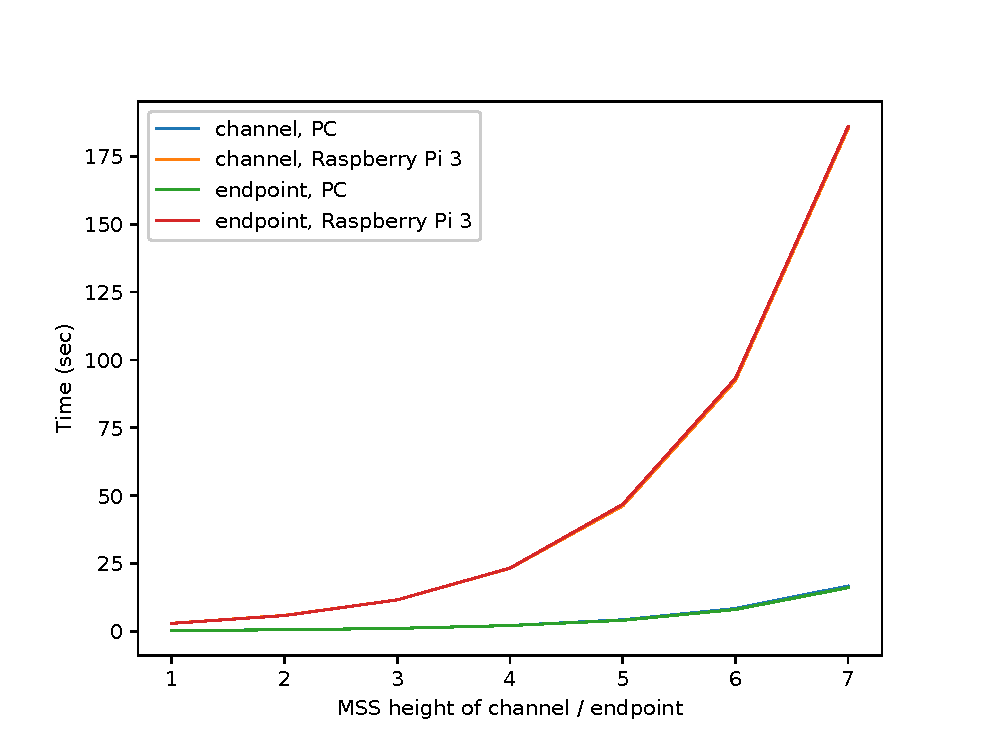
\includegraphics[width=2.5in]{mam_create}
    \caption{Time cost of MAM creation.}
    \label{fig:mam_create}
\end{figure}

\subsubsection{Messages Publishment}
Publishing a message to MAM is attaching a zero-value transaction to the Tangle which requires two processes:
\begin{itemize}
	\item	Tips selection: In the IOTA protocol, a new-coming transaction needs to pick up 2 existed transactions called tips to reference and verify. The tips are provided by IOTA full nodes.
	\item	Proof-of-Work (PoW): An algorithm which prevents Denial of Service and spam attacks on a network. A computationally hard puzzle to solve, but easy to verify. IOTA uses a Hashcash\cite{Hashcash} based puzzle.
\end{itemize}

Tips selection requires a stable network connection to wait the response from IOTA full nodes, and PoW requires enough computation resources to perform. Fig.~\ref{fig:mam_send} shows probability distribution function of publishing a message to MAM endpoint. The time of Raspberry Pi 3 distributed widely, since the randomness of PoW has huge impact while all the tests on PC remain in a possible range.

\begin{figure}[!t]
    \centering
    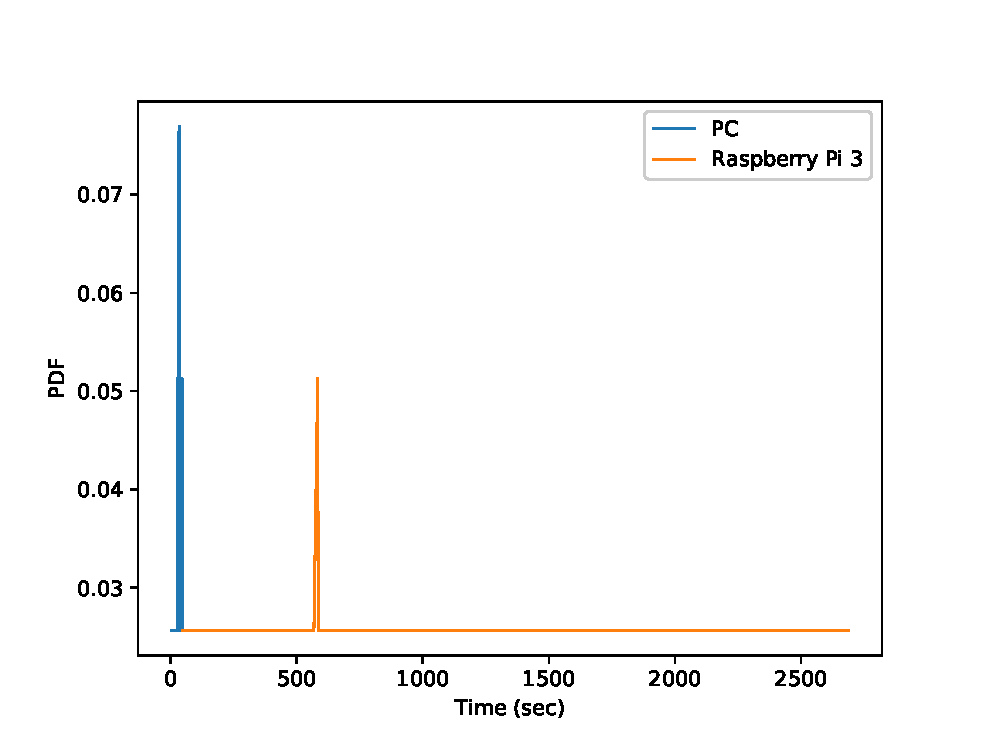
\includegraphics[width=2.5in]{mam_send}
    \caption{Time cost of sending a message through MAM.}
    \label{fig:mam_send}
\end{figure}

The simulation results above indicate that MAM is difficult for low-level sensor devices to run, whereas these kind of devices are the majority hardware in the IoT scenarios. Furthermore, sensors with the low computing power and unstable internet connection are not able to have enough resources to handle data collection, data transmission on MAM and even trading process with subscribers simultaneously. 

Therefore, transferring MAM operations to brokers while ensuring the profit and privacy of providers through blind signatures can effectively solve performance problems and lower the threshold to participate in such framework. Brokers can be PCs or powerful machines that runs Ethereum client and Tangle-accelerator\cite{TA}. Where Ethereum client is used to interact with Ethereum and Tangle-accelerator is a caching proxy server for IOTA, which can serve thousands of IOTA requests at once without accessing remote IOTA full nodes frequently and provide PoW acceleration. Fig.~ \ref{fig:ta_struct} shows the structure of Tangle-accelerator. However, MAM operations still cost a considerable time that improving the performance of MAM is an essential issue that needs to be done for the next step.  

\begin{figure}[!t]
    \centering
    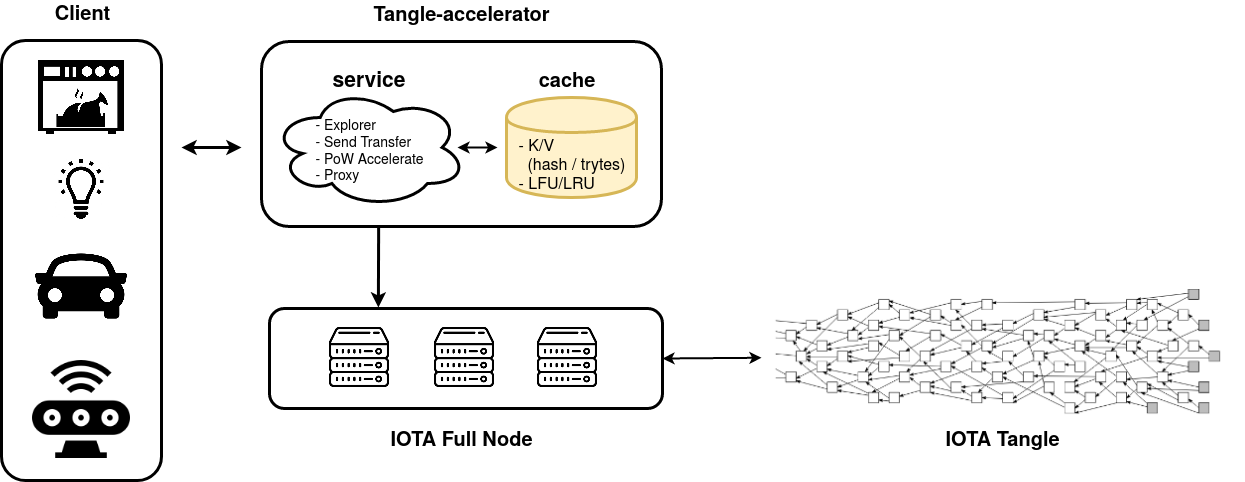
\includegraphics[width=3in]{ta_structure}
    \caption{The structure of Tangle-accelerator.}
    \label{fig:ta_struct}
\end{figure}

\section{Conclusions}
By combining the established standards and openly-developed specifications, this paper proposed an autonomous publish/subscribe model design to serve as a vendor and industry-neutral platform, automating the trading of digital assets and services. It was built with blockchain network, immutable audit trails, and contracts with an integrated decentralized identity system, to ensure the authenticity of all participants and enable secure communication and flexible trading mechanisms.

\bibliographystyle{IEEEtran}
\bibliography{references}

\end{document}
